\documentclass[a4paper,11pt,onecolumn,twoside]{article}
\usepackage{ctex}
\usepackage{times}
\usepackage{setspace}
\usepackage{fancyhdr}
\usepackage{graphicx}
\usepackage{subfigure}
\usepackage{multicol}
\usepackage{wrapfig}
\usepackage{array}  
\usepackage{fontspec,xunicode,xltxtra}
\usepackage{titlesec}
\usepackage{titletoc}
\usepackage[titletoc]{appendix}
\usepackage[hyphens]{url}
\usepackage{cite}
\usepackage{listings}
\usepackage[framed,numbered,autolinebreaks,useliterate]{mcode} % 插入代码
\XeTeXlinebreaklocale "zh"
\XeTeXlinebreakskip = 0pt plus 1pt minus 0.1pt

\lstset{basicstyle=\footnotesize\ttfamily,breaklines=true, language=bash, xleftmargin=2em, xrightmargin=1em,  aboveskip=1em}
  

%%%%%%%%%%%%%%%%%%%%%%%%%%%%%%%%%%%%%%%%%%%%%%%%%%%%%%%%%%%%%%%%
%  lengths
%    下面的命令重定义页面边距,使其符合中文刊物习惯。
%%%%%%%%%%%%%%%%%%%%%%%%%%%%%%%%%%%%%%%%%%%%%%%%%%%%%%%%%%%%%%%%
\addtolength{\topmargin}{-54pt}
\setlength{\oddsidemargin}{-0.9cm}  % 3.17cm - 1 inch
\setlength{\evensidemargin}{\oddsidemargin}
\setlength{\textwidth}{17.00cm}
\setlength{\textheight}{24.00cm}    % 24.62


%%%%%%%%%%%%%%%%%%%%%%%%%%%%%%%%%%%%%%%%%%%%%%%%%%%%%%%%%%%%%%%%
% 标题,作者,通信地址定义
%%%%%%%%%%%%%%%%%%%%%%%%%%%%%%%%%%%%%%%%%%%%%%%%%%%%%%%%%%%%%%%%
\songti
\title{\huge{“跳房子”智能教具的设计与实现}
% \thanks{收稿日期:~XXXX$-$XX$-$XX.i.}
\thanks{基金项目:2016南京大学本科教学改革重点课题(201616B1);南京大学“十三五”实验教学改革研究课题(SY201904);国家级大学生创新创业训练计划资助项目(G201810284028)}
\thanks{通信作者:张志俭(1976- ),男,学士,高级工程师,研究方向:嵌入式系统、物联网技术、创新创业教育}
}
\author{石广钊\quad 张志俭\quad 宋坤\quad  谭博文\quad 杨紫薇\quad 周文涛\\[2pt]
\normalsize
(南京大学电子科学与工程学院, 江苏省~南京市~211046) \\[2pt]}
\date{}  % 这一行用来去掉默认的日期显示


%%%%%%%%%%%%%%%%%%%%%%%%%%%%%%%%%%%%%%%%%%%%%%%%%%%%%%%%%%%%%%%%
% 首页页眉页脚定义
%%%%%%%%%%%%%%%%%%%%%%%%%%%%%%%%%%%%%%%%%%%%%%%%%%%%%%%%%%%%%%%%
% \fancypagestyle{plain}{
% \fancyhf{}
% \lhead{第~XX~卷\quad 第~X~期\\
% \scriptsize{XXXX~年~XX~月}}
% \chead{\centering{X~~X~~X~~期~~刊\\
% \scriptsize{\textbf{The trip to get the Sutra}}}}
% \rhead{Vol. XX, No. XX\\
% \scriptsize{October, 2004}}
% \lfoot{}
% \cfoot{}
% \rfoot{}}

%%%%%%%%%%%%%%%%%%%%%%%%%%%%%%%%%%%%%%%%%%%%%%%%%%%%%%%%%%%%%%%%
% 首页后根据奇偶页不同设置页眉页脚
% R,C,L分别代表左中右,O,E代表奇偶页
%%%%%%%%%%%%%%%%%%%%%%%%%%%%%%%%%%%%%%%%%%%%%%%%%%%%%%%%%%%%%%%%
% \pagestyle{fancy}
% \fancyhf{}
% \fancyhead[RE]{第~XX~卷}
% \fancyhead[CE]{西~~天~~取~~经~~记}
% \fancyhead[LE,RO]{\thepage}
% \fancyhead[CO]{猴~~哥等:王母娘娘寿筵上蟠桃生长过程仿真与分析}
% \fancyhead[LO]{第~X~期}
% \lfoot{}
% \cfoot{}
% \rfoot{}

\makeatletter
\newenvironment{figurehere}
  {\def\@captype{figure}}
  {}
  % \newcommand\figcaption{\def\@captype{figure}\caption}
  % \newcommand\tabcaption{\def\@captype{table}\caption}
\makeatother


%---------------------------------------------------------------------
%	引用文献设置为上标
%---------------------------------------------------------------------
\newcommand{\supercite}[1]{\textsuperscript{\cite{#1}}}

\begin{document}
\maketitle

%%%%%%%%%%%%%%%%%%%%%%%%%%%%%%%%%%%%%%%%%%%%%%%%%%%%%%%%%%%%%%%%
%%%%%%%%%%%%%%%%%%%%%%%%%%%%%%%%%%%%%%%%%%%%%%%%%%%%%%%%%%%%%%%%
%  中文摘要
%  调整摘要、关键词,中图分类号的页边距
%  中英文同时调整
%%%%%%%%%%%%%%%%%%%%%%%%%%%%%%%%%%%%%%%%%%%%%%%%%%%%%%%%%%%%%%%%
\setlength{\oddsidemargin}{ 1cm}  % 3.17cm - 1 inch
\setlength{\evensidemargin}{\oddsidemargin}
\setlength{\textwidth}{13.50cm}
\vspace{-.8cm}
\begin{center}
\parbox{\textwidth}{
\heiti 摘~~~要\quad \kaishu~传统游戏丰富多彩,对孩子很有益处,而智能玩具则玩法多样,能够引起孩子兴趣。从传统游戏“ 跳房子”出发,设计了游戏模式多样、拓展性强的智能教具。系统以CC2530控制单个格子,外加压力探测、LED灯提示模块构成跳房子节点;以树莓派为总体控制核心,外加音乐播放、触摸屏模块构成主机。灯光、音乐提示增加了游戏的趣味性,通过触摸屏可自定义游戏则使游戏智能化。\\
\heiti 关键词\quad\kaishu 智能玩具;跳房子;ZigBee;树莓派;幼儿教育\\
\heiti 中图分类号\quad TS958.28\qquad  \heiti 文献标识码\quad B}
\end{center}
%%%%%%%%%%%%%%%%%%%%%%%%%%%%%%%%%%%%%%%%%%%%%%%%%%%%%%%%%%%%%%%%
%  英文摘要
%%%%%%%%%%%%%%%%%%%%%%%%%%%%%%%%%%%%%%%%%%%%%%%%%%%%%%%%%%%%%%%%
\vspace{.1cm}
\begin{center}
\parbox{\textwidth}{
{\large{\textbf{Design and Implementation of "Talling House" Intelligent Teaching Aid}}}\\
\vspace{-0.5cm}
\begin{center}
\textbf{ShiGuangzhao\quad ZhangZhijian\quad SongKun\quad TanBowen\quad YangZiwei\quad ZhouWentao}\\[2pt]
\small{\textit{(School of Electronic Science and Engineering, Nanjing Univ., Nanjing Jiangsu 211046, China)}}\\[2pt]
\end{center}
{\small{\textbf{Abstract}\quad Traditional games are rich and colorful, which is good for children, while smart toys have a variety of ways to play, which can arouse children's interest. Starting from the traditional game "hopscotch", we have designed intelligent teaching aids with diverse game modes and strong expansion. The system controls a single grid with CC2530, plus pressure detection and LED light prompt module to form a hopscotch node; the Raspberry Pi is the overall control core, plus music playback and touch screen modules form the host. Lights and music tips add to the fun of the game, and customizing the game through the touch screen makes the game smart. \\
\textbf{Key Words}\quad Intelligent toys; Hopscotch; ZigBee; Raspberry pie; Early childhood education.}}
}
\end{center}


%%%%%%%%%%%%%%%%%%%%%%%%%%%%%%%%%%%%%%%%%%%%%%%%%%%%%%%%%%%%%%%%
%  文章编号(左上角)
%%%%%%%%%%%%%%%%%%%%%%%%%%%%%%%%%%%%%%%%%%%%%%%%%%%%%%%%%%%%%%%%
% \begin{minipage}[c]{10cm}
% \vspace{-35.5cm}
% 文章编号~~~~1005$-$0388(2004)05$-$0505$-$04
% \end{minipage}

%%%%%%%%%%%%%%%%%%%%%%%%%%%%%%%%%%%%%%%%%%%%%%%%%%%%%%%%%%%%%%%%
%  恢复正文页边距
%%%%%%%%%%%%%%%%%%%%%%%%%%%%%%%%%%%%%%%%%%%%%%%%%%%%%%%%%%%%%%%%
\setlength{\oddsidemargin}{-.5cm}  % 3.17cm - 1 inch
\setlength{\evensidemargin}{\oddsidemargin}
\setlength{\textwidth}{17.00cm}
%%%%%%%%%%%%%%%%%%%%%%%%%%%%%%%%%%%%%%%%%%%%%%%%%%%%%%%%%%%%%%%%
%  分栏开始
% \begin{multicols}{2}

\begin{spacing}{1.2}
\songti
    % \zihao{-4}

\section{引言}
    传统游戏丰富多彩,蕴含着几千年来人类的教育智慧\supercite{1}。对于孩子们而言,民间传统游戏不仅仅是传统文化的传承,更重要的是提高他们的学习能力、认知能力以及合作能力。以民间游戏“ 跳房子”为例,跳房子游戏不但能让孩子动起来,从而提高身体素质,而且对于培养孩子的规则意识、合作能力以及创新能力有极大地帮助\supercite{2,3}。但随着时代的变化,早期的传统游戏已经不能满足当代孩子们对于玩具们的要求了\supercite{6}。相比之下,既有趣味性又有创新挑战性的智能玩具能更好的激发孩子们的兴趣。但我国目前智能玩具研究中存在低水平、多重复、创新少等问题\supercite{4},适合幼儿的智能玩具较少,智能玩具\supercite{7}应用环境有限。同时,目前我国的智能玩具更多偏重于培养儿童认知能力,而较少关注动作技能以及交际能力的培养\supercite{8}。

    跳房子智能教具的设计从传统游戏“跳房子“出发,开发出一种包含智能玩具和传统游戏优点的新型智能玩具。在此智能教具中,格子通过LED灯光来确定游戏基本规则-灯光颜色来决定格子能否被踩。同时,控制中心播放相应的音乐,并在显示屏上显示。跳房子智能教具中,游戏者可通过预先自定义来设定游戏者在游戏中的路径,且系统支持单脚或双脚模式,单人或多人游戏,满足游戏者对游戏的自主创新和拓展的需求\supercite{4,10}。此外系统还开发出了演奏模式,可使孩子以跳跃的方式独奏或合奏乐曲,具有较强趣味性。系统格子数量可变,具有较强的拓展性。

\section{系统整体方案}
    系统主要由主机模块和多个节点模块构成,系统框图如图\ref{fig:kuangtu}所示。主机模块以树莓派(Raspberry Pi 3B+)作为控制中心,游戏开始前游戏者通过触摸屏选择或自定义游戏模式,树莓派通过CC2530协调器完成与CC2530节点之间的无线通信(ZigBee),即接收节点状态以及向节点发送指令,并根据节点状态控制扬声器播放相应音乐并在显示器上显示。其中单个节点由一个 CC2530 单片机控制,当游戏程序设定该节点应该被踩下时,节点控制 LED 模块发出相应灯光,提示游戏者节点应该被踩下,同时通过压力传感器探测节点是否被踩下,并将状态发送至主机模块。

\begin{figure}[htb]
    \centering
    {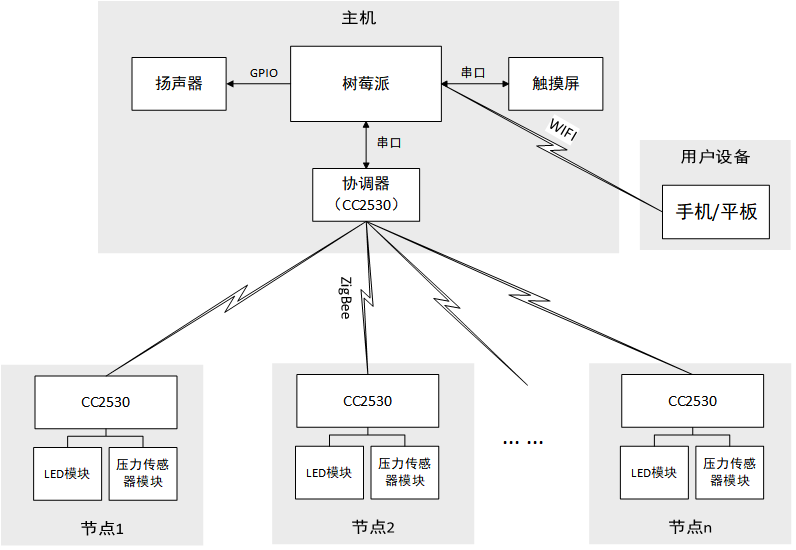
\includegraphics [width=0.5\textwidth]{./image/框图V3.png}
    \caption{系统框图}
    \label{fig:kuangtu}}
\end{figure}

   系统在传统跳房子游戏基础上做了极大的创新,系统包含多种游戏模式并支持游戏者对于游戏模式的自定义,不同年龄阶段的孩子通过不同的游戏模式培养和增强与该年龄阶段应有的能力\supercite{5}。

    以本系统应用于在幼儿教学中的应用为例。对于 3-4 岁幼儿,游戏主要是在教师的带领下完成。游戏开始前由教师通过触摸屏或手机 APP 选择游戏模式,之后主机将预设的游戏信息通过 ZigBee 网络发到各节点,节点收到信息后点亮 LED 模块,通过不同背景颜色提示参与者该节点是否应该被踩下,红色代表不可踩,蓝色代表可踩。幼儿根据颜色提示跳跃踩踏格子,当节点探测到踩踏后通过 ZigBee 无线通信将节点编号和踩踏时间传递给主机,主机收到节点编号后对照预设数据并记录时间,如果踩对则控制扬声器发出美妙乐音,如果踩错则发出鼓励话语。以此方式引导幼儿完成整个游戏过程,培养低龄幼儿的动作协调和学习能力,并在游戏中培养起孩子的规则意识。

    而对大龄幼儿游戏则更加丰富,可以选择单脚还是双脚进行游戏,并且可以由孩子自定义格子踩下的路径,能够很好培养该阶段儿童的创新能力和动手能力,也能够满足当下幼儿传统课程设计的需求\supercite{4}。在闯关竞争模式下,节点控制 LED 模块点亮时间,时间到则提示光关闭,要求大龄幼儿快速记住可踩踏格子的位置,每组成员在完成游戏后以准确率和完成速度进行打分,对培养幼儿的竞争意识和合作能力有较好作用。

    此外,系统还支持音乐模式,即使单个节点对应音乐中的一个音,通过踩下按照提示踩下节点,即可“弹奏”出相应的乐曲,如果踩错则会发出不一样的声音,不同节奏的乐曲可以适应不同年龄阶段的幼儿。通过独奏或合奏乐曲,让孩子在游戏中感受音乐,对孩子态度情感方面\supercite{9} 能力的培养有很大益处,同时通过合奏乐曲也能培养孩子的合作能力和协调能力\supercite{11}。

\section{硬件系统设计}
    系统主要由一个主机模块和多个节点模块构成,主机作为整个游戏进程的控制中心,完成与用户的交互功能,包含树莓派、协调器和音乐播放模块,并通过连接到触摸屏或用户手机 APP;节点作为跳房子的格子,完成探测状态和提示用户路径的功能,包含压力传感器模块和 LED 模块。

    \subsection{主机模块}
    \subsubsection{树莓派模块}
    系统主机所采用的树莓派(Raspberry Pi 3B+)具有主频 1.4GHz 的 64 位四核 ARM Cortex-A53CPU,内置 1G 内存,具有很好的计算性能。内置 WiFi 和蓝牙 4.2,方便手机端控制整个系统。主机程序建立在 Raspberry Pi 中嵌入的 Linux 系统上,使得主机程序能够更加智能化,且稳定性、流畅性较好,同时也使得更为丰富的游戏模式的开发成为可能\supercite{12}。

    Raspberry Pi 提供了包括 HDML、GPIO 等丰富的接口,具有很强的拓展性,本系统中通过 GPIO 将树莓派与协调器和扬声器相连,可完成相互之间的通信,而通过显示器接口则可连接到触摸屏,通过 WiFi 网络可为手机 APP 提供连接。

    \subsubsection{协调器模块}
    ZigBee 技术是一种短距离、低功耗的无线通信技术,具有很好的性能,在当今物联网领域得到了大量的应用\supercite{13}。本系统采用 ZigBee 协议完成主机模块与节点模块之间的无线通信。

    CC2530 结合了有业界领先的 RF 收发器性能的增强型 8051CPU,系统内可编程闪存,拥有 8kB RAM,CC2530 搭载德州仪器 ZigBee 协议栈($Z-Stack^{TM}$ ),提供了强大的 ZigBee 解决方案。本系统节点和协调器均以 CC2530 为平台,并通过 ZigBee 协议进行组网和通信\supercite{14}。协调器的作用是协调主机与节点之间的通信,进行信息中转和转换。

    系统中协调器以中断方式接收从主机通过串口发来的消息并将其通过协议栈向节点广播,而各个节点则以单播的方式向协调器发送信号,协调器通过串口将信息发至主机。


    \subsubsection{音乐播放模块}
    通过简谱可以得到乐曲中各个音的调号、发音的顺序以及各个音的长短,而乐曲中每个音所对应的频率是固定的,如C调中音do频率为523Hz,且每两个半音频率之比为$\sqrt[2]{12}$。通过使树莓派引脚输出相应频率方波到扬声器,即可获得相应声音,由此系统根据简谱即可“演奏”出完整的乐曲。系统通过调用wiringPi函数库实现对树莓派GPIO口的控制。

    由于树莓派输出电流太大会导致系统关机甚至损坏开发板,故设计扬声器电路如图\ref{fig:yangshengqi}所示,扬声器通过外接电源供电,树莓派引脚只需输出高低电平。由于三极管输入电阻很大,树莓派在音乐播放模块输出电流很小,能够防止系统因电流过大而损坏。

\begin{figure}[htb]
    \centering
    {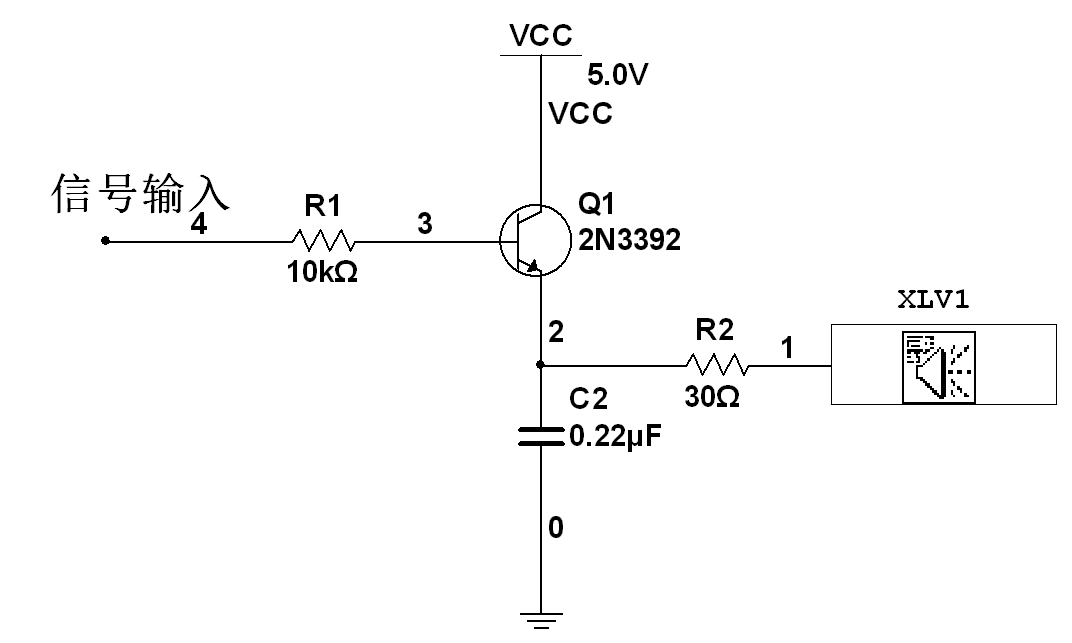
\includegraphics [width=0.5\textwidth]{./image/music.png}
    \caption{扬声器电路}
    \label{fig:yangshengqi}}
\end{figure}

\subsection{节点模块}
    \subsubsection{单片机模块}
    作为无线传感网络节点,CC2530具有很好的性能\supercite{15}。本系统节点由CC2530单片机控制。系统定义引脚P0\_1用于控制LED灯亮灭,当P0\_1输出高电平时,LED灯亮起,当输出为低电平时,LED灯熄灭;压力传感器用于判断是否被踩下,未被踩下时,其向端口输出高电平,传感器被踩下后输出变为低电平,将压力传感器输出引脚接到CC2530的某个引脚上(如P0\_3),节点单片机便可据此判断节点是否被踩下。
    节点PCB板电路如图\ref{fig:pcb}所示。

\begin{figure}[htb]
    \centering
    {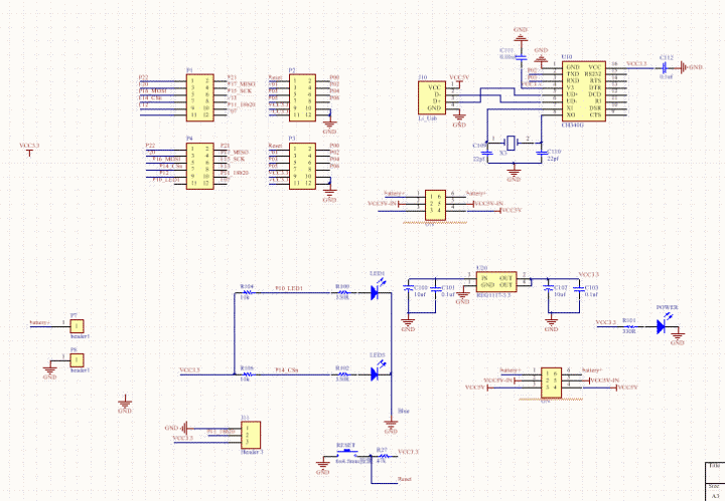
\includegraphics [width=0.5\textwidth]{./image/pcb2.png}
    \caption{节点电路}
    \label{fig:pcb}}
\end{figure}

    \subsubsection{LED模块}
    LED 模块接收节点 CC2530 信号并以此决定是否发光以及发出何种灯光,为了达到较好的效果,系统通过采用多个 LED 并联以使显示效果更加明显,为了增强趣味性,LED模块能够根据程序显示出不同的形状。

    \subsubsection{压力传感器模块}
    压力传感器模块由于探测节点是否被踩下,并将之传至节点单片机引脚。

    此处用到压力传感器可通过调节其上的旋钮改变触发所需的最小压力,此处我们设置为10kg,以防止抖动导致传感器的误判。

    通过在格子的各个角落放置传感器,可以获取游戏者平衡状态,主机由此能够判断幼儿平衡能力并在显示器上显示。


\section{系统软件设计}

\subsection{树莓派模块}
    树莓派(主机)模块是整个游戏的计算中心,同时也承担着控制显示器和控制音乐播放的任务。此部分程序采用C语言写成,其中音乐播放用到的引脚以及与协调器交互用到的串口收发通过调用wiringPi 函数库实现,显示界面采用gtk+ 作为开发平台,为了让音乐播放以及图形的显示不影响与协调器的交互,这里也采用了多线程pthread库实现各个功能部分的分离。

    wiringPi 是Raspberry Pi 中较为常用的 IO 控制库,使用C语言开发,并提供了C语言和 Python 等的接口,能够很好的满足本系统需求。gtk+ 是GNU/Linux 环境下主流的图形开发环境之一,提供了大量C语言接口。

    主机简略流程图如图\ref{fig:liucheng}所示。

    树莓派内嵌入Linux系统,开机后系统运行“跳房子”游戏程序。开始游戏后程序将建立游戏线程,用户完成节点初始化和模式初始化 ,即可开始游戏。完成模式选择后,程序将为模式新建一个不分离线程。游戏过程中主机根据从协调器收到的信息判断踩对与否,从而调用不同函数实现声音提示,同时在显示屏上显示,游戏中用户可点击菜单栏实现重新初始化。
 
\begin{figure}[htb]
    \centering
    {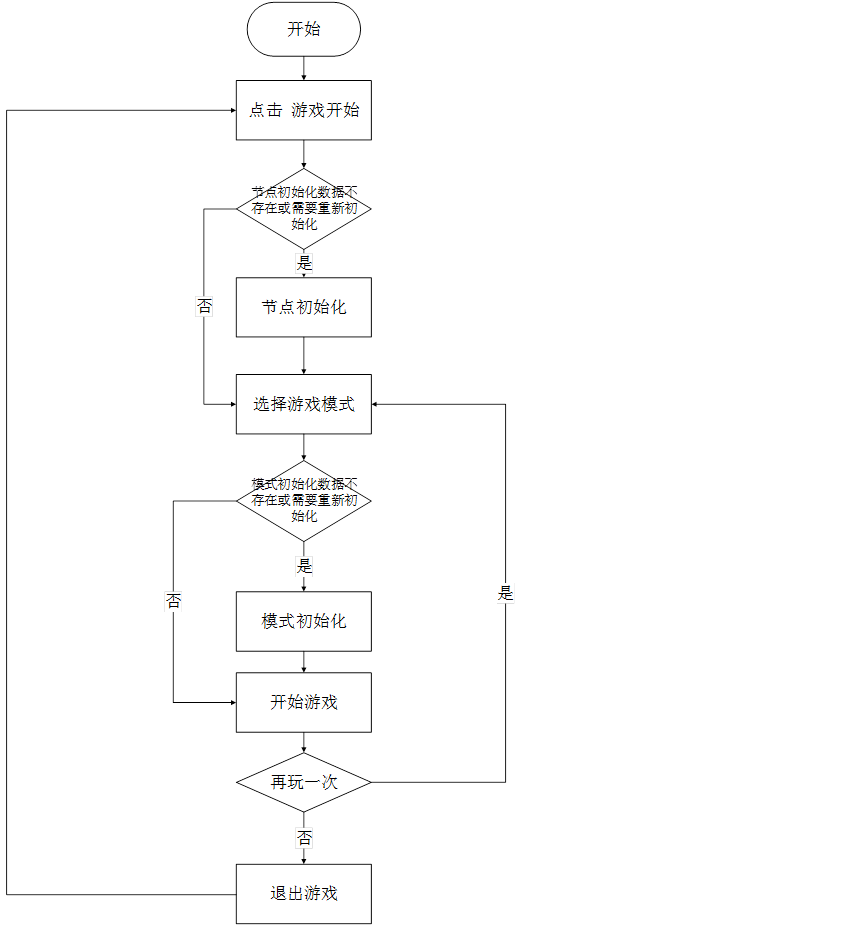
\includegraphics [width=0.5\textwidth]{./image/流程图.png}
    \caption{主机程序流程图}
    \label{fig:liucheng}}
\end{figure}

    通过调用pthread\_cancel( ) 函数取消模式线程或游戏线程,就能够实现重新选择游戏模式或退出游戏,程序中设置两个全局变量用于检测用户通过菜单进行的音效设置,相应控制游戏音效和结束音效。

 \subsection{节点模块}
    系统节点和协调器所使用的单片机均为由 TI 公司生产的 CC2530 单片机,节点和协调器之间的 ZigBee 通信正是建立在 TI 的 Z-Stack 协议栈之上。

    系统定义每个节点 ID 为一个字节的数,即 C 语言中一个 char 类型的变量。系统首次开机初始化时,结合用户的配合节点可获取到各自的 ID,并将之写入非易失电存储区(NV)中,之后无需再次初始化。

    节点以中断方式接收协调器信号,如与自身 ID 相同,表示节点应该被踩下,LED 模块亮起以给出提示。同时查询压力传感器状态,如果被踩下则以单播方式向协调器发送节点 ID。协调器发送从主机收到的信息给节点,发送从节点收到的信息给主机,协调器起的就是“翻译”和缓冲的功能,于是协调器中设置了串口接收中断和 RF 接收中断,相应中断处理函数即通过协议栈或串口发送信息给另一端。

\section{总结}
    “跳房子”智能教具利用树莓派平台使得传统的跳房子游戏变得“智能化”,可通过自定义增加游戏操作的多样性,使其能供更大年龄范围的人使用;而ZigBee无线通信技术则使格子可移动、可拓展,使游戏玩法能够更加多样;同时通过声音、图像以及灯光的提示加强孩子对于游戏的专注度。此运动教具既保留了原有游戏的趣味性,能让孩子动起来,又使游戏智能化,吸引孩子注意力,锻炼孩子的智力、身体协调能力以及协作能力。并且该智能教具对教育创新有很大的支持。它可以丰富孩子们初级阶段的兴趣活动,也为幼儿园小学等提供了更多种多样的教学方式,创设更加愉快的教学氛围[17]。

    “跳房子”智能教具不仅继承和发展了民间传统游戏,刺激孩子们对更多的传统游戏产生兴趣,并且很好的吸收了智能玩具在提高孩子们创新能力方面的优点,同时对于孩子认知能力、动作技能以及交际能力的培养提供了很好的方法,能够很好的填补市场上相关产品的空缺。

\end{spacing}

%%%%%%%%%%%%%%%%%%%%%%%%%%%%%%%%%%%%%%%%%%%%%%%%%%%%%%%%%%%%%%%%
%  参考文献
%%%%%%%%%%%%%%%%%%%%%%%%%%%%%%%%%%%%%%%%%%%%%%%%%%%%%%%%%%%%%%%%
\small
\begin{thebibliography}{99}
\setlength{\parskip}{0pt}  %段落之间的竖直距离
\bibitem{1}李姗泽.学前教育应重视中华民族优秀传统文化——论民间游戏在幼儿园课程资源中的地位和作用[J].课程.教材.教法,2005(05):31-35.
\bibitem{2}杨频.“跳房子”游戏在小学校园内课间体育活动中的作用[J].湖南医科大学学报(社会科学版),2010,12(02):258-259.
\bibitem{3}李翠红. 跳房子游戏促进大班幼儿合作能力的研究 [J]. 课程教育研究, 2014(16):8.
\bibitem{6}焦奕.忻州市民间传统体育游戏衰落的成因分析[J].体育科技文献通报,2017,25(10):134-136.

\bibitem{4}王海霞. 小学体育《跳房子》教学设计与反思 [J]. 新课程研究 (基础教育),2009(04):48-49.
\bibitem{7}周艳,李青.我国智能玩具研究现状述评——基于2002—2014年中文文献[J].北京邮电大学学报(社会科学版),2016,18(01):113-120.
\bibitem{10}周晨光. 再谈用新材料翻新 拓展经典老游戏 [J]. 体育教学, 2016,36(09):74.
\bibitem{8}王嘉琦, 张运锋. 电子商务环境下智能玩具产业的现状及对策分析 [J]. 电子商务, 2012(10):6-8.
\bibitem{5}马来祥. 民间儿童游戏对儿童发展的促进作用分析——以河南民间游戏 “跳房子” 为例 [J]. 中国校外教育, 2014(36):57.
\bibitem{9}李青, 周艳. 智能玩具: 助推教育创新的新技术 [J]. 远程教育杂志, 2016,34(01):46-52.
\bibitem{12}王凯巍, 孙康, 张子伊, 陈美娟, 朱晓荣. 基于 ZigBee 与树莓派的环境信息采集系统 [J/OL]. 实验科学与技术: 1-6[2018-12-05].http://kns.cnki.net/kcms/detail/51.1653.N.20180706.1603.048.html.
\bibitem{13}李俊斌, 胡永忠. 基于 CC2530 的 ZigBee 通信网络的应用设计 [J]. 电子设计工程, 2011,19(16):108-111.
\bibitem{11}李淑君. 浅谈幼儿音乐教育中音乐与游戏交互作用的意义 [J]. 大众文艺, 2018(22):217-218.
\bibitem{14}王风. 基于 CC2530 的 ZigBee 无线传感器网络的设计与实现 [D]. 西安电子科技大学, 2012.
\bibitem{15}章伟聪, 俞新武, 李忠成. 基于 CC2530 及 ZigBee 协议栈设计无线网络传感器节点 [J]. 计算机系统应用, 2011,20(07):184-187+120.



% \bibitem{chuanchen}罗红辉.民间传统儿童游戏的传承与创新[J].学前教育研究,2014(11):67-69.
% \bibitem{youeryuan}彭海蕾. 幼儿园游戏教学研究 [D]. 西北师范大学, 2002.


% \bibitem{cheche}彭卫东, 周超. 具有语音和图像识别及跟踪功能的智能玩具车设计 [J]. 科学技术与工程, 2012,12(16):3880-3884.
% \bibitem{xiaoche}董胡,马振中.基于单片机的智能玩具小车设计[J].微型电脑应用,2014,30(09):14-16.
% \bibitem{wanju}海广, 李洪鹏, 余震. 基于 arduino 单片机控制的无线儿童玩具设计及可视化实现 [J]. 科技创业月刊, 2013,26(04):193-196.

\end{thebibliography}
{
\zihao{-5}
\noindent {\heiti 作者简介:}

\noindent {\heiti 石广钊}(1998- ),男,本科,电子信息科学与技术专业。通信地址:南京市栖霞区仙林大道163号,211046,Tel:18851827330,E-mail:GuangZhao\_Shi@163.com.
}

% \end{multicols}
\end{document}
